%%%%%%%%%%%%%%%%%%%%%%%%%%%%%%%%
\section{Detector monitoring and slow control}
\label{sec:slowcontrol}

The scope of the ProtoDUNE-SP detector control system (DCS) includes the design, procurement, fabrication, testing,
and delivery
of a comprehensive detector monitoring, control and safety system.

The responsibility for the system is split between ProtoDUNE-SP and CERN: 
\begin{itemize}
\item	The ProtoDUNE-SP collaboration is responsible for all the devices that will be installed and cabled inside 
the cryostat, the sensors needed to monitor the cryostat and its content, and the specifications for the system. % needs. 
\item	CERN is responsible for the implementation of the control system elements outside the cryostat (hardware, firmware and software), including the high-voltage and low-voltage power supplies necessary for the detector operation.
\end{itemize}

This section describes %the monitoring devices and sensors inside the cryostat, 
the main requirements, 
constraints and assumptions of the control system, and its general structure and components. 

%%%%%%%%%%%%%%%%
\subsection{Monitoring devices and sensors}
A number of %monitoring 
devices and sensors will be located inside the cryostat for either periodic or continuous monitoring of %detection of some fundamental parameters of 
the LAr as well as the GAr in the ullage, %content 
and for the monitoring of the detector functionality.

\fixme{A short section on requirements here would be useful}

%%%%%%%%%
\subsubsection{Purity Monitors} 
Three purity monitors (PrM) with sensitivity in the ppt range will be used for the direct determination of the impurity content of the LAr inside the ProtoDUNE-SP cryostat. These PrMs have been generously provided by ICARUS~\cite{Ica-PrM-TM} after being decommissioned from the T600. The design has been replicated for MicroBooNE and other R\&D test experiments at FNAL. Inside the ProtoDUNE-SP the monitors are arranged in a single vertical string located behind the APA planes on the Jura side (see Figure~\ref{fig:cryo-side-names}). The string hangs from the large blanking flange on the manhole, and ports with ConFlat sealing on the blanking flange will be made available for HV/Signal/OptFiber feedthroughs. The string is about 7~m long, with the three PrMs strung at different heights: one near the LAr surface, one at mid-height, and one at the very bottom near the LAr-return manifold, %for the return LAr distribution 
for monitoring the purity of the LAr entering the cryostat after the filtration process.  

\begin{cdrfigure}[A purity monitor from ICARUS T600 ]{IcaPrM.pdf}{Picture of a purity monitor from the ICARUS T600, now available for installation in the ProtoDUNE-SP detector}
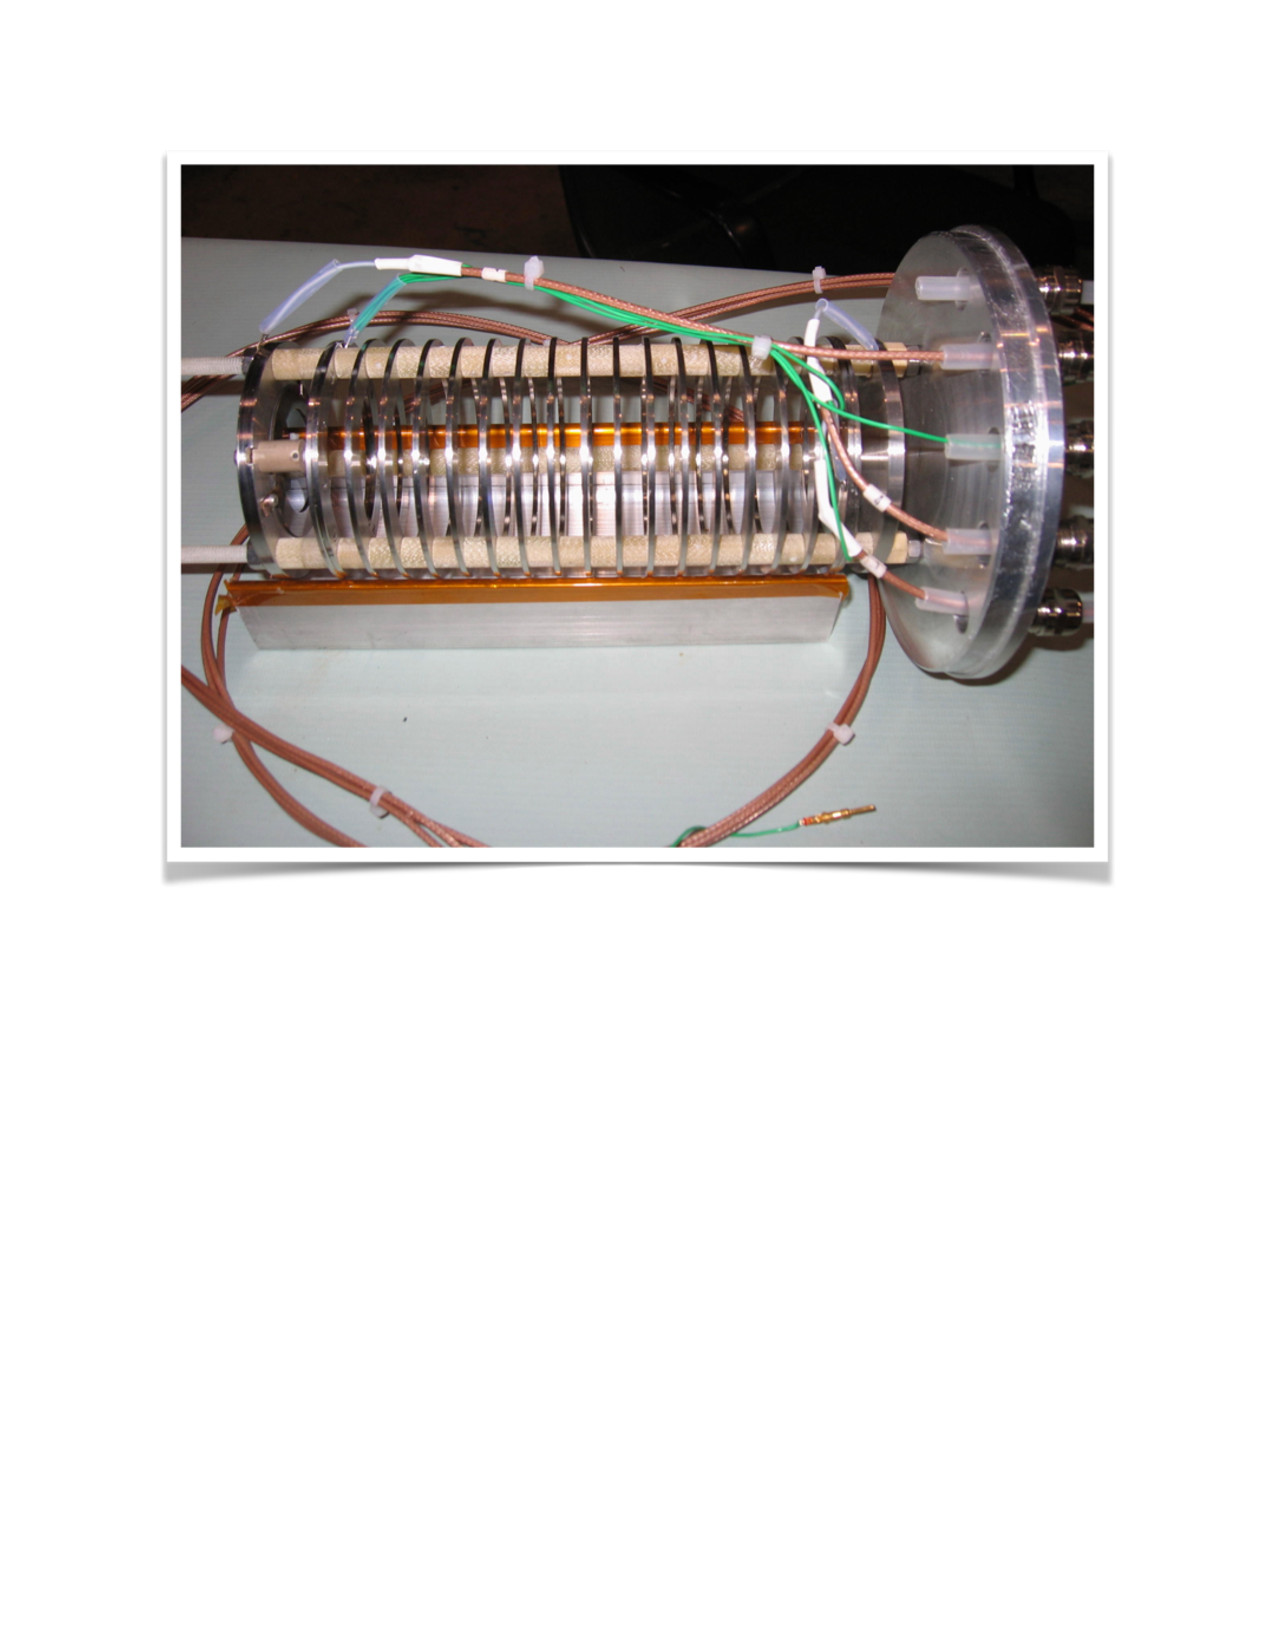
\includegraphics[width=0.5\textwidth]{IcaPrM.pdf} 
\end{cdrfigure}

\fixme{ Figure \ref{fig:IcaPrM} was not referenced; I added one. It's pretty, but not very informative. It could use more description like ``the 16(?) divisions in the device are the whatever, and the connection on the right is ...'' Or we could take it out.}

The three PrMs, one of which is pictured in Figure~\ref{fig:IcaPrM}, are currently being refurbished with new gold photocathode and new quartz fiber. The drift length  (25~cm) is the same for all them. Using parts of another (available) PrM to extend the drift length of one of the three (e.g., to 40~cm) for more precise measurements of the longer $e-$ lifetimes is currently %considered as an open option.
under consideration.
The mechanical structure of the string, the anchorage to the manhole flange at the top end, and the fastening of the string at the bottom %are subject of a detailed ongoing engineering study. 
are still under study.
An additional PrM at the bottom on the opposite side of the cryostat would be useful for %comparing 
%with the response from the other PrM at the same height and thus 
%checking %the uniformity of 
monitoring variations in the quality of 
the LAr at that level, and providing information for the fluid-dynamics computation inside the cryostat. \\

%%%%%%%%%
\subsubsection{Vertical Temperature Gradient Monitor}

	Precise monitoring of the temperature gradient as a function of LAr depth is %considered highly important as 
	an important input for fluid dynamics modeling and simulations. The installation of a set of devices with precision better than 50~mK
	%the precise measurement of the LAr temperature across 
	along the entire height of the LAr volume %inside the cryostat 
	has recently  been included in the internal instrumentation plan  for this purpose.
%	A precision better than 50~mK in the temperature measurement is assumed as target requirement for the device. 
	Commercial calibrated resistance temperature detectors (RTDs -- Pt100 or Pt1000) with 15-mK precision at LAr temperature are well suited to this application, however the temperature probe wiring and signal transport outside the cryostat require extreme care in order to maintain % is necessary to prevent spoiling 
	the intrinsic precision of the probe.
	
The %current base option  
design for this device consists of a series of 25 Pt100 probes positioned at $\sim$30~cm intervals %distance between one another 
along a $\sim$7.5-m-long rigid string hanging behind the APA plane from %the flange %on one of 
an available port %on the top side 
at the top of the cryostat. A special multi-pin FT is mounted on the flange %is necessary 
for the signal extraction and readout from a temperature controller.  
Again, the mechanical structure, including the cable routing up to the multi-pin FT, is still subject to a detailed engineering study.
%Also in this case, the engineering study of the mechanical structure has to be developed in detail, including cables routing up to the multi-pin FT. \\
A number of RTDs will also be positioned on the APAs and on the cryostat walls at different heights to monitor the temperature %drop 
during the cooling process. %phase.

%%%%%%%%%
\subsubsection{Webcams}
	Based on %the solution 
	a system developed by ETH Zurich for WA105, six commercial webcams, sealed inside a specially developed metal case with a ConFlat optical window to allow operation at cryogenic temperatures, are located inside the cryostat. They are positioned at strategic points allowing inspection of the interior during filling and commissioning, % operations, 
	and detection (and recording) of possible sparks in locations exposed to high %the highest 
	electric field intensity.
	
%%%%%%%%%
\subsubsection{Level Meters}
	Reliable LAr level determination is required in the $\pm$20~cm around the nominal LAr surface level. Commercially available liquid-level sensors provide high-reliability monitoring. These are available in multiple technologies, %y types, 
	including solid-state electro-optical, %conductivity, 
	conductive, capacitive and piezo-resonant. Although the technology choice has not been made%yet, however 
	designated ports on the top of the cryostat are available for this instrumentation.
The vertical temperature gradient device will provide a coarse level reading during filling and 
 a differential pressure transducer will also provide additional indication about LAr level.
 
 \fixme{the temp gradient device provides ``coarse'' measurement, but this device provides ``reliable'' measurement, not ``precise'' measurement. Pls clarify}

%%%%%%%%%
\subsubsection{Pressure Sensors}
	Precise measurement of pressure in the GAr ullage is necessary. A number of pressure sensors, including a differential pressure transducer, are planned, %foreseen 
	and designated ports on the top of the cryostat are available for this instrumentation.

%%%%%%%%%%%%%%%%
\subsection{Slow Control System}

The design of the ProtoDUNE-SP safety and control system is largely based on the experience gained in collaboration with ETH Zurich during the pilot WA105 project at CERN. The components of this system and their functions are as follows:
\begin{itemize}
\item	The Process Control System (PCS) reads temperature sensors including the Vertical T Gradient monitor, pressure sensors and the purity monitors inside the cryostat and the trace analyzers (O$_2$, N$_2$, H$_2$O) in the external recirculation line.
\item	The Detector Control System (DCS) monitors and controls the low voltage (LV) and high voltage (HV) from the power supplies.
\item	The Detector Safety System (DSS) %ensures the safety of the experiment by 
performs temperature surveys and monitors interlocks.
\end{itemize}
The system provides a graphical user interface to visualize the trends of monitored values, the alarms, and to control the \fixme{operation of the?} experiment. A web interface allows remote monitoring of the behavior of the experiment. 
\fixme{relating `control the experiment' and `monitor behavior of experiment,' it seems out of order. Can you start with monitor and then say control?}

The physical interface of the control system is located at the level of the outer flanges on the cryostat. \fixme{Where is this shown?}
% While 
 CERN EP/DT-DI will take care of connecting the control system to the flanges and interfacing to the cryogenics control infrastructure for information and signal exchange. 
The ProtoDUNE-SP experiment is responsible for all sensors, power distribution, etc., inside the cryostat, % are part of the experiment's responsibilities 
as well as for defining the system specifications, I/O parameters and control \& safety logics. \fixme{logic or logistics?}
 
The supervisory control of the system and data acquisition (SCADA) will be developed, tested and provided by CERN EP/DT-DI.	%CERN will develop and test the SCADA supervisor for ProtoDUNE-SP.
\fixme{still `will be developed'?}

Figure \ref{fig:dcsdesign} shows the general architecture of the control and safety system for ProtoDUNE-SP, including the PCS, the DCS and the DSS.
%The system is subdivided into the Process Control System, the Detector Control System and the Detector Safety System described above.

\begin{cdrfigure}[DCS design]{dcsdesign}{Proposed architecture and technical solution of the control and safety system.}
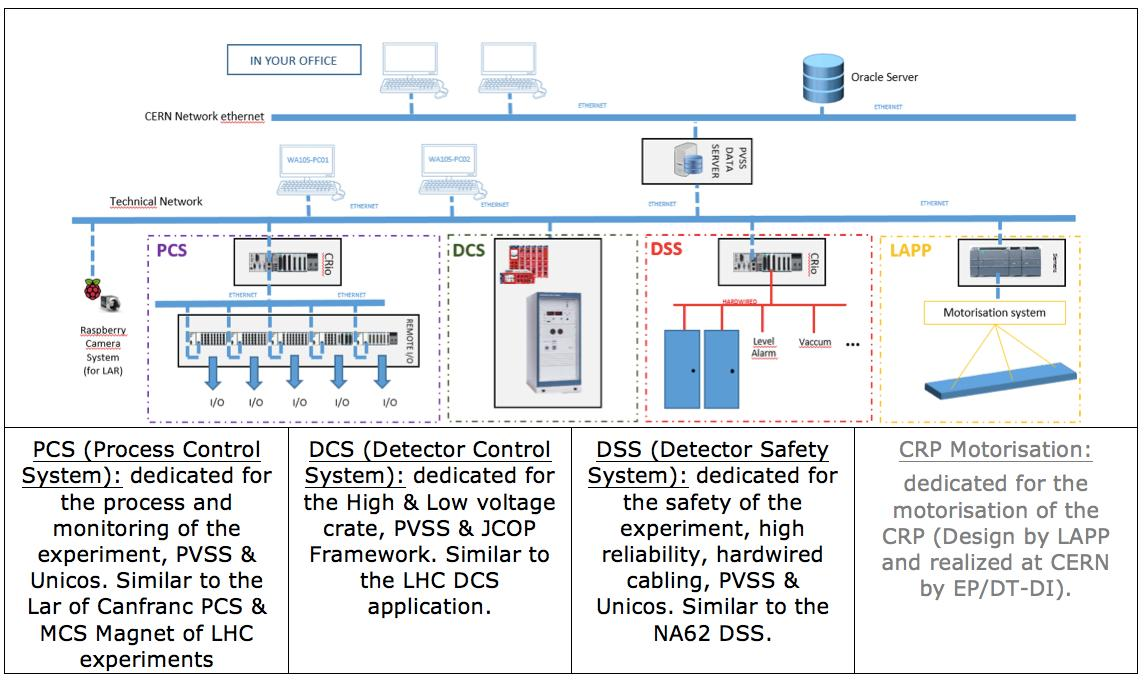
\includegraphics[angle=90, height=0.9\textheight]{DCS_Design}
\end{cdrfigure}

The control system is composed of:
\begin{itemize}
\item a chassis for electrical distribution (380~Vac, 220~Vac, 24~Vdc redundant);
\item two chassis for the PCS, composed of an FPGA, signal conditioners, interface, and cabling;
\item  one chassis for the DCS,  composed of an interface for LV/HV monitoring \& control; 
\item a chassis for the DSS, composed of an FPGA and relays for the safety of the experiment; 
\item a chassis for a PC data acquisition \& supervision (PVSS SCADA Supervisor), composed of a computer with a display monitor, a switch and a server; 
\item four chassis for the remote I/O to capture signals close to the detector and to avoid multi-cabling structure; and
\item  one chassis for the HV, controlled by the slow-control system. 
\end{itemize}
All these elements will be mounted in 19-in. racks.

The supervisory software is based on the JCOP framework, an integrated set of software tools originally developed for the control of the LHC experiments at CERN and now used in several more experiments at CERN. Besides providing a supervisory control and data acquisition system, the framework offers many tools for the implementation of finite state machines, archival of data, as well as graphical interfaces as web dashboards.

